
\subsection{Implementace komunikace se serverem}
V této kapitole se detailněji podíváme na implementaci komunikace se serverem.

\begin{figure}[tbh!]
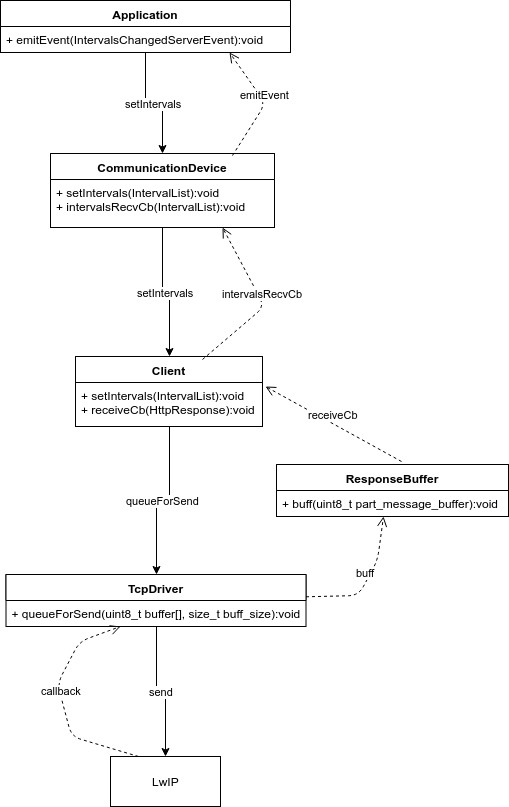
\includegraphics[width=\textwidth, height=600px]{../diagrams/stm_implementace_komunikace.jpg}
\caption{Diagram tříd v rámci komunikace}
\label{stm-implementace-komunikace}
\end{figure}

% popis skupiny Communication
V diagramu \ref{stm-implementace-komunikace} jsou zobrazeny nejdůležitější třídy, vztahy
mezi nimi a zároveň je tam zobrazen i typický proces nastavení intervalů na STM a stažení
intervalů ze serveru, který bude popsán později.
Nejprve popíšeme třídy v diagramu a jejich funkcionalitu.
\begin{itemize}
  \item \texttt{CommunicationDevice} který je objektovou reprezentací samotného STM a \texttt{Application}
    do ní ukládá naměřenou teplotu pro odeslání na server a intervaly pro výměnu se serverem.
    CommunicationDevice notifikuje Application o dvou důležitých událostech - \texttt{ConnectedEvent} a
    \texttt{IntervalsChangedServerEvent} - tedy připojení k serveru a přijetí intervalů ze serveru.
  \item \texttt{Client} je HTTP klientem specifickým pro naše použití. Jednak do něj CommunicationDevice
    přeposílá data, které má od Application, a jednak Client notifikuje CommunicationDevice o
    důležitých událostech týkajících se komunikace se serverem jako jsou: \uv{intervaly byly odeslány},
    \uv{teplota byla odeslána}, \uv{intervaly byly přijaty}, apod.
  \item \texttt{TcpDriver} je wrapper pro LwIP knihovnu.
  \item \texttt{ResponseBuffer} reprezentuje buffer pro HTTP odpovědi ze serveru.
    TcpDriver přeposílá vše, co přijme, do ResponseBuffer.
    Ten si tato data ukládá dokud nedostane celou HTTP zprávu.
    Typicky se totiž stává, že server neodešle celou HTTP odpověď v jednom paketu a proto je potřeba
    jednotlivé pakety ukládat a později z nich poskládat celou HTTP odpověď.
    V momentě, kdy ResponseBuffer má celou odpověď, notifikuje o tom Clienta.
    ResponseBuffer také potřebuje vědět jestli očekávaná odpověď od serveru má mít i tělo nebo pouze
    HTTP hlavičku.
\end{itemize}

% popis vztahů
Směrem dolů od Application až po LwIP probíhá odesílání dat na server resp. zařazení těchto dat
do interních front LwIP - k samotnému odeslání dat typicky dojde později.
Směrem nahoru od LwIP, přes TcpDriver, ResponseBuffer až po Application probíhá příjem dat
ze serveru.
Z pohledu kódu se dá směr dolů považovat za \uv{synchronní} a směr nahoru za \uv{asynchronní}, proto
jsou také všechny metody, které jsou volané směrem nahoru, definovány jako callback metody.

% popis procesů znázorněných na diagramu
Na diagramu jsou znázorněny dva typické procesy:

\paragraph{Posílání intervalů na server}
Proces probíhající směrem dolů bychom mohli nazvat jako \uv{uložení intervalů do interních
struktur Clienta k budoucímu porovnání s intervaly serveru} (porovnávat se ve skutečnosti bude
pouze timestamp intervalů).
Jakmile se intervaly dostanou do Clienta, musí zde Client počkat, dokud se jeho \emph{komunikační cyklus}
(zmíněný dále v této kapitole) nedostane do stavu, ve kterém porovnává timestamp svých intervalů
a timestamp intervalů ze serveru.
Nezávisle na tom, jak toto porovnání dopadne, musí Client poslat buď GET request, nebo POST request
na server přes TcpDriver.

\paragraph{Příjem intervalů ze serveru}
Je proces probíhající směrem nahoru.
LwIP předává přijatý payload TCP paketů do TcpDriver, který ho dále předává do ResponseBuffer.
Jak již bylo zmíněno, ResponseBuffer postupně ukládá části HTTP odpovědi, dokud nesestaví celou,
potom notifikuje Client pomocí callback metody.
ResponseBuffer už HTTP odpověď naparsoval a Client na základě toho, v jakém stavu \emph{komunikačního cyklu}
se nachází, notifikuje CommunicationDevice (na diagramu notifikuje CommunicationDevice o přijetí
intervalů ze serveru pomocí callback metody \texttt{intervalsReceivedCb}).
CommunicationDevice dále vygeneruje \texttt{IntervalsChangedServerEvent} a pošle do Application
k následnému šíření.

% Client
\subsubsection{Client}
Kromě toho že Client je HTTP klientem, musí také být implementován tak, aby byl kompatibilní s LwIP
callback API.

\begin{figure}[tbh!]\centering
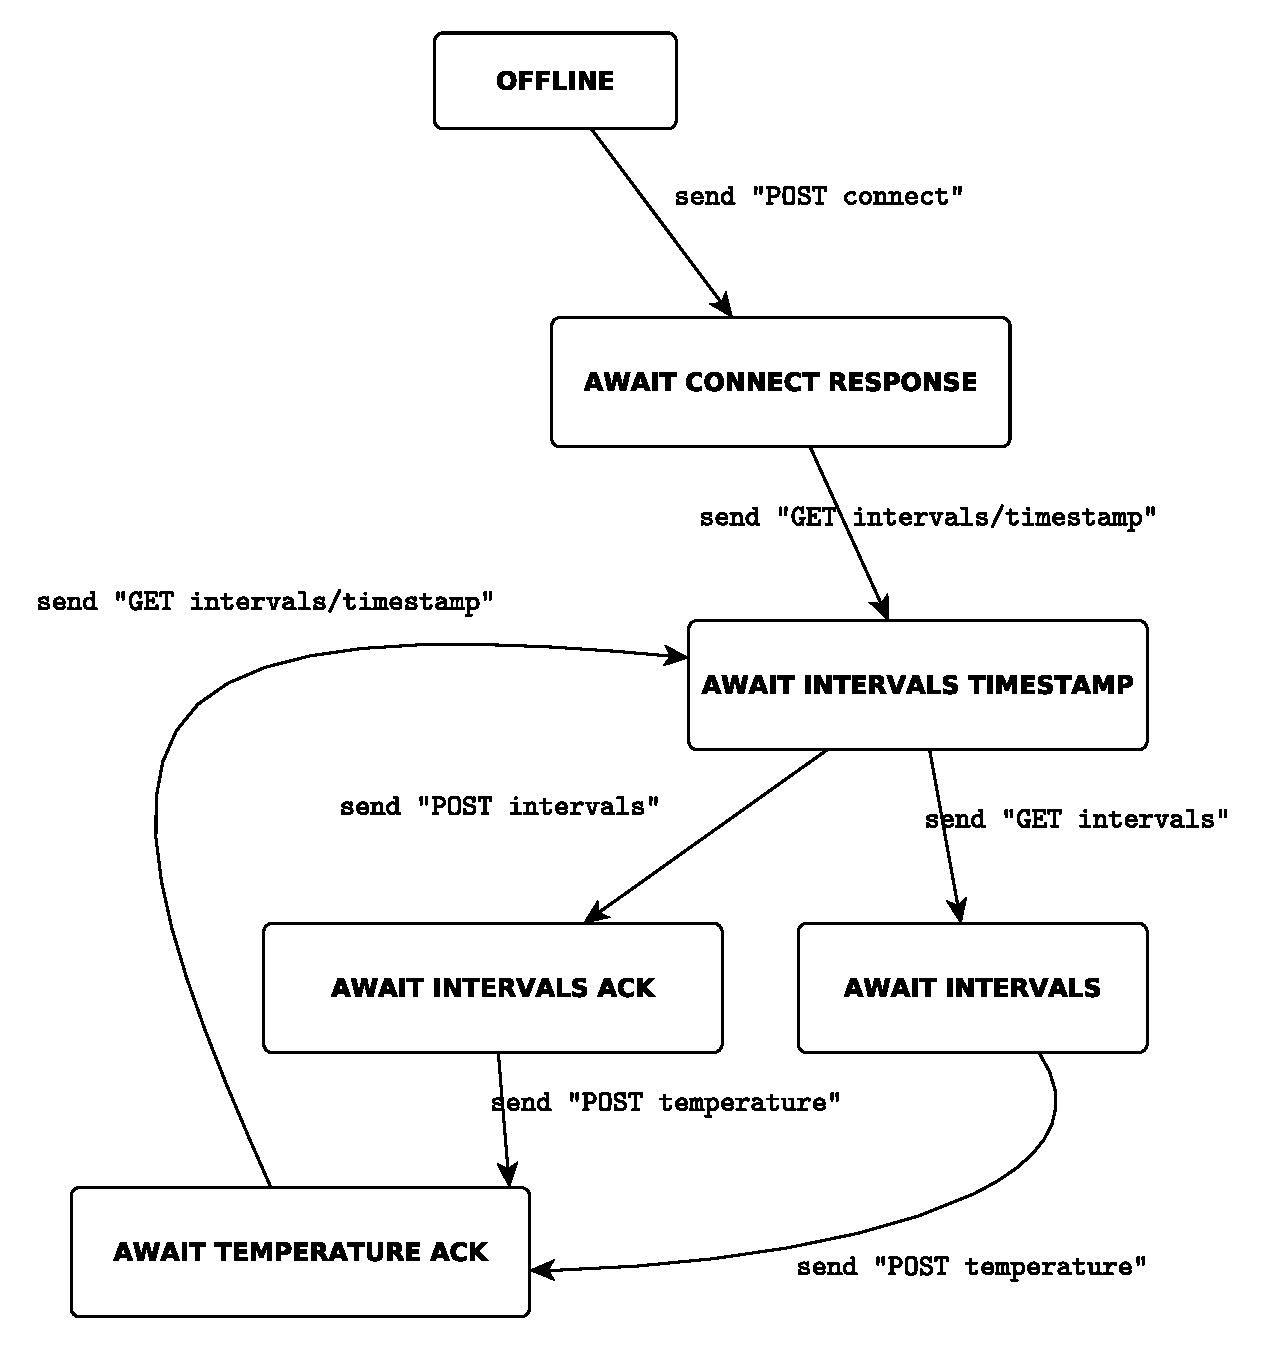
\includegraphics[width=\textwidth, height=150mm]{../diagrams/stm_komunikacni_cyklus.pdf}
\caption{Komunikační cyklus}
\label{stm-komunikacni-cyklus}
\end{figure}

Na diagramu \ref{stm-komunikacni-cyklus} je znázorněn \emph{komunikační cyklus} a jednotlivé stavy tohoto cyklu.
Zjednodušeně řečeno se v rámci celého cyklu nejprve buď pošlou intervaly na server nebo stáhnou ze
serveru - záleží na tom, jestli má STM větší timestamp než server - poté se pošle teplota na server.
Pokud cyklus probíhá poprvé, musí se nejprve STM k serveru přihlásit.
Celý cyklus je opakován v určitých časových intervalech.
\footnote{Konkrétně jsou to 2 sekundy, je pro to použit softwarový časovač}

% Ošetření chyb
Mezi libovolnými dvěma stavy může dojít k chybě.
Chyby ošetříme tak, že celý cyklus restartujeme od stavu \texttt{OFFLINE}.
Mohli bychom sice uložit stav před chybou a po zpracování chyby pokračovat opět od tohoto stavu,
bylo by to ale příliš komplikované.
Navíc v našem případě je během celého cyklu přeneseno relativně malé množství dat, takže restartování
od úplného začátku nás skoro nic nestojí.


